%
% Section 3
%
\section{App}

\begin{frame}{App - Wahl des Frameworks: Nativ?}
	\centering
	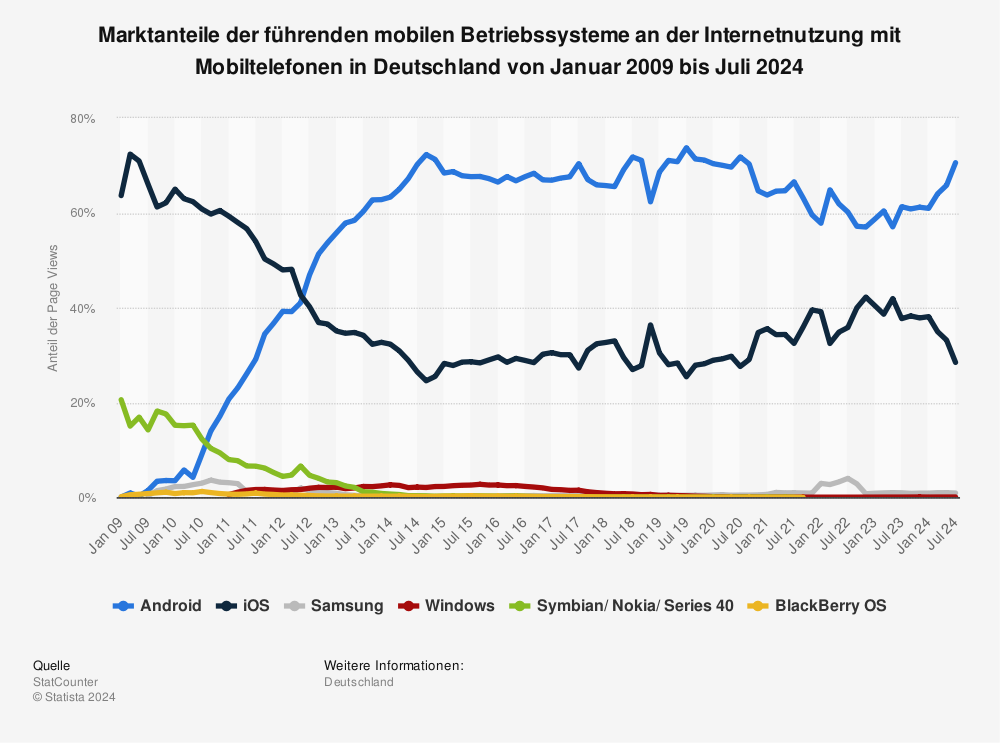
\includegraphics[height=0.9\textheight]{images/app/flutter/statista_mobile.png}
	\cite{StatistaMobil}
\end{frame}

\begin{frame}{App - Wahl des Frameworks: Cross Platform?}
	\centering
	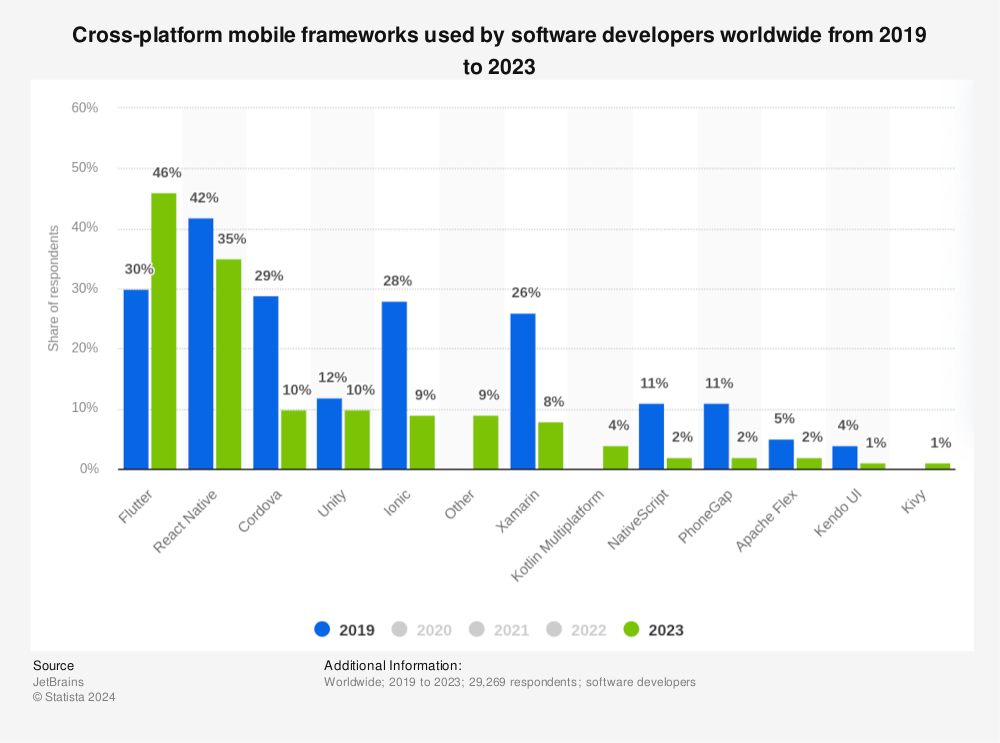
\includegraphics[height=0.9\textheight]{images/app/flutter/cross_platform_statista.png}
	\cite{StatistaCross}
\end{frame}

\begin{frame}{App - Flutter}
	\centering
	\begin{itemize}
		\item Eigene Rendering-Engine
		\item Deklarativer Ansatz
		\item Widgets: Stateless oder Stateful
		\item Programmiersprache Dart für UI und Logik
		\item Aktive Weiterentwicklung von Flutter und Dart
		\item Große/Wachsende Communty
	\end{itemize}
\end{frame}

\begin{frame}{App - Flutter: Dart}
	\centering
	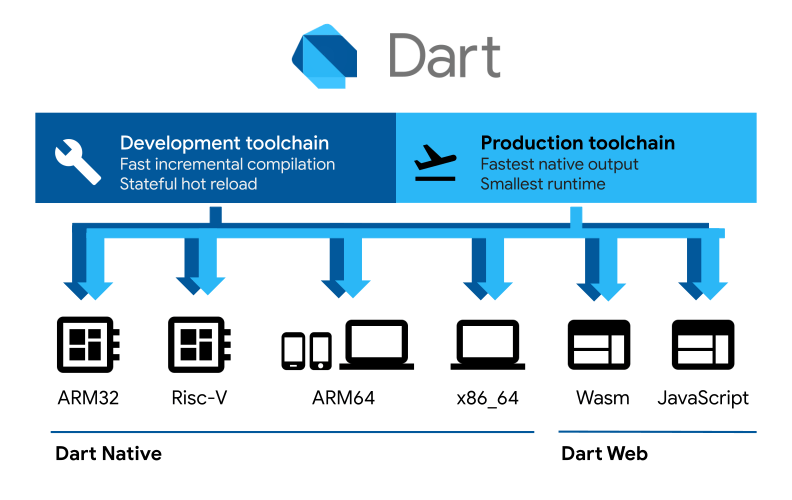
\includegraphics[height=1.0\textheight]{images/app/flutter/dart-diagram-small}
	\cite{darttoolchains}
\end{frame}

\begin{frame}{App - Flutter: Dart}
	\centering
	\begin{itemize}
		\item Strong Typing mit Sound Null Safety
		\item Bundled Package Manager pub
		\item Viel syntaktischer Zucker
		\item Pattern Matching, Mixins, Records u.v.m.
	\end{itemize}
\end{frame}

\begin{frame}{App - Kommunikation mit Server}
	\begin{itemize}
		\item Kommunikation mit Server über REST-API
		\item 19 API Endpunkte
	\end{itemize}
	\centering
	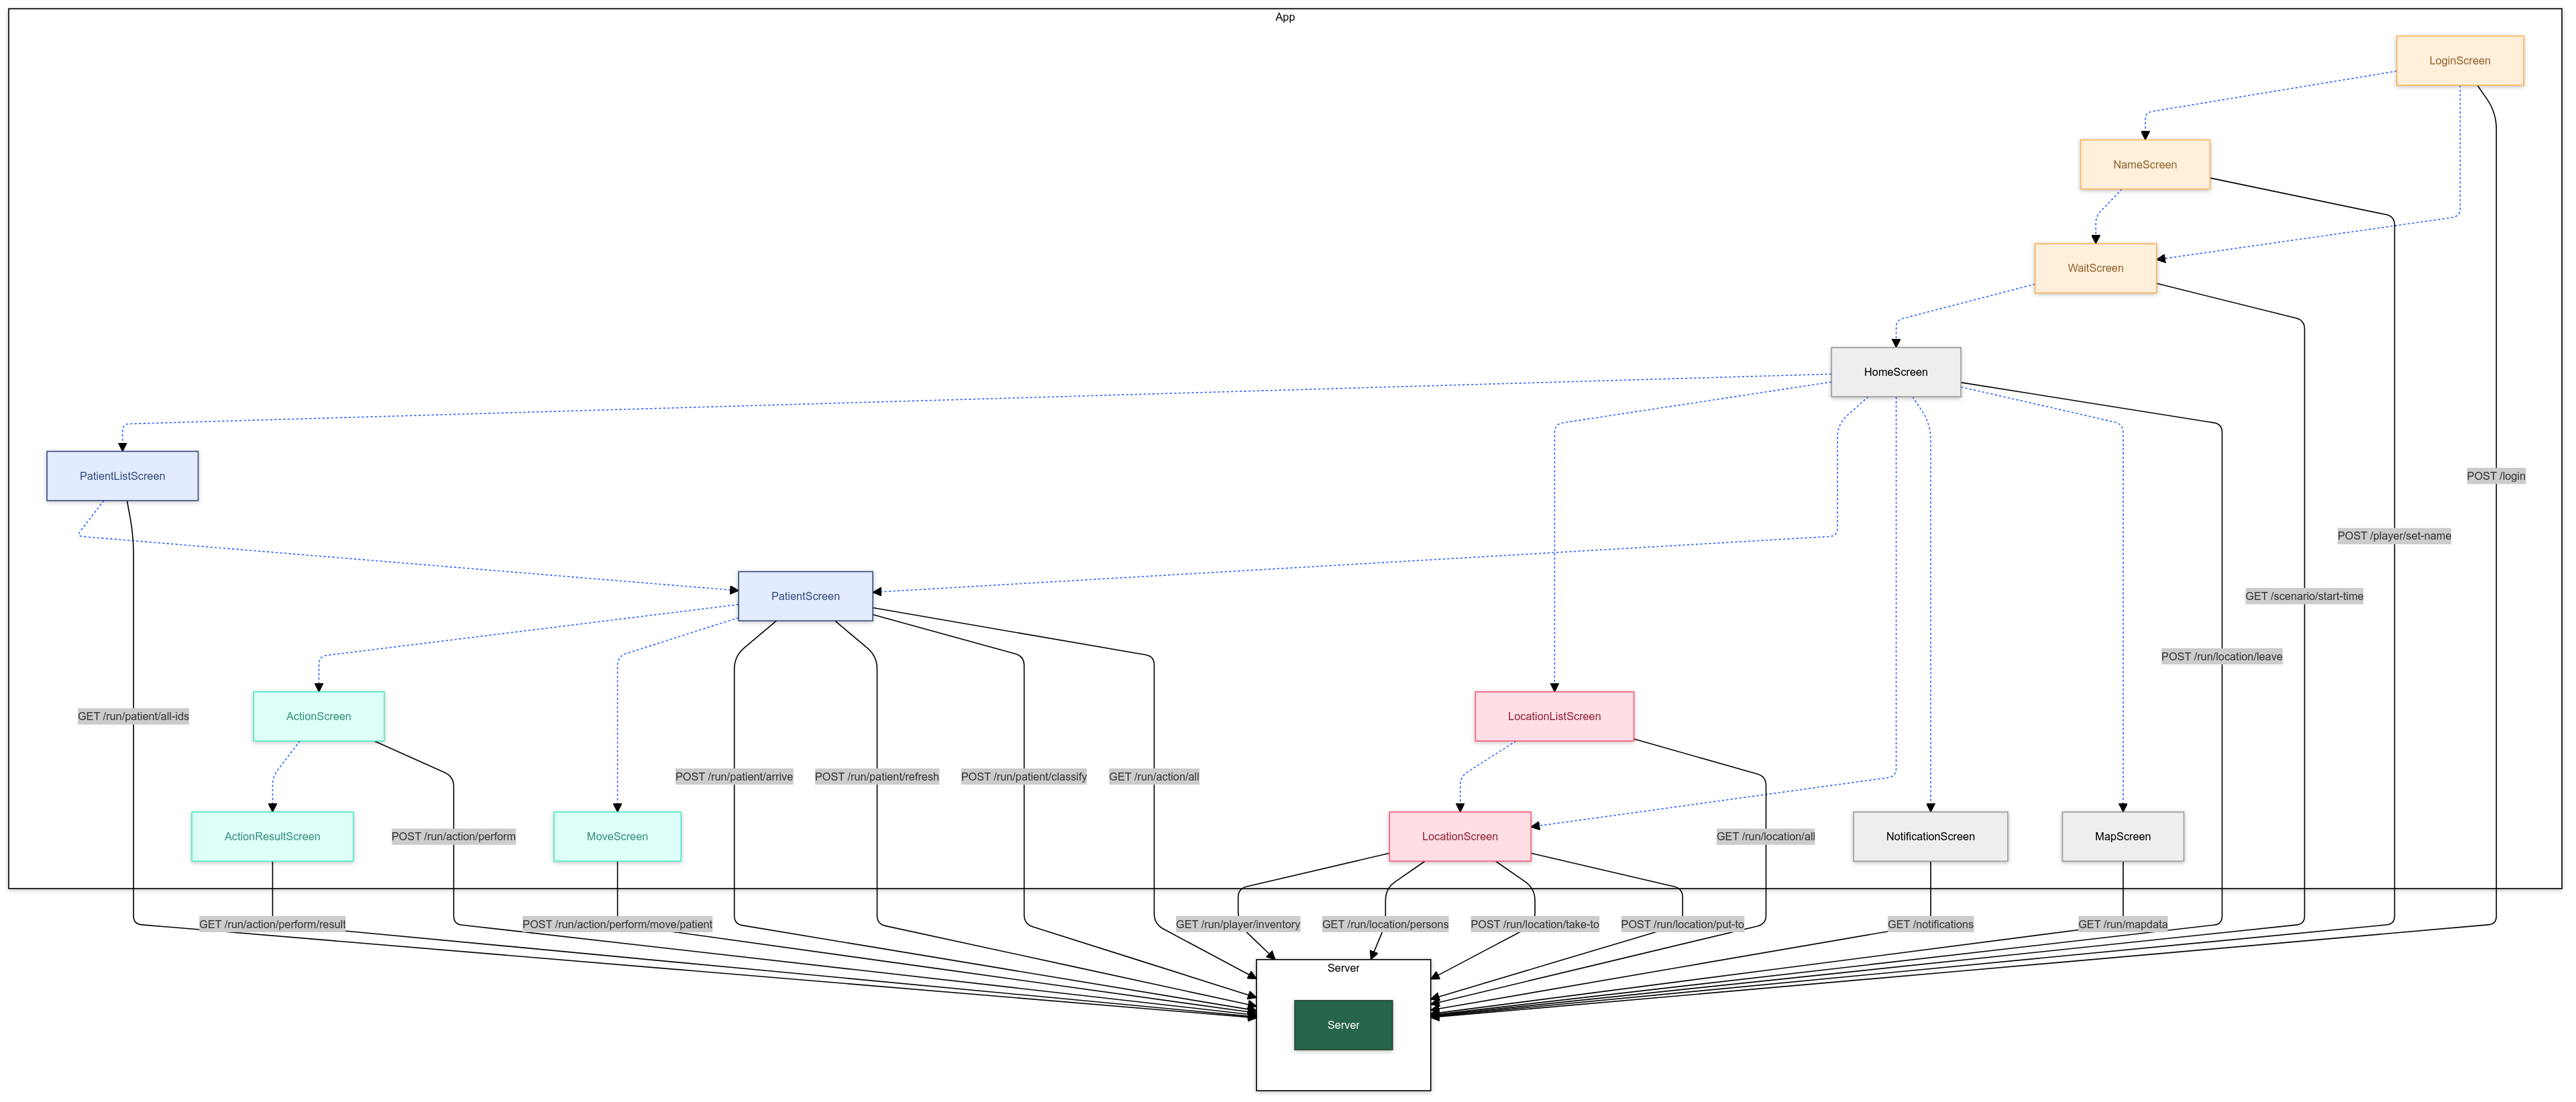
\includegraphics[width=1.0\textwidth]{images/app/server_endpoints.png}
\end{frame}

\begin{frame}{App - Kommunikation mit Server}
	\centering
	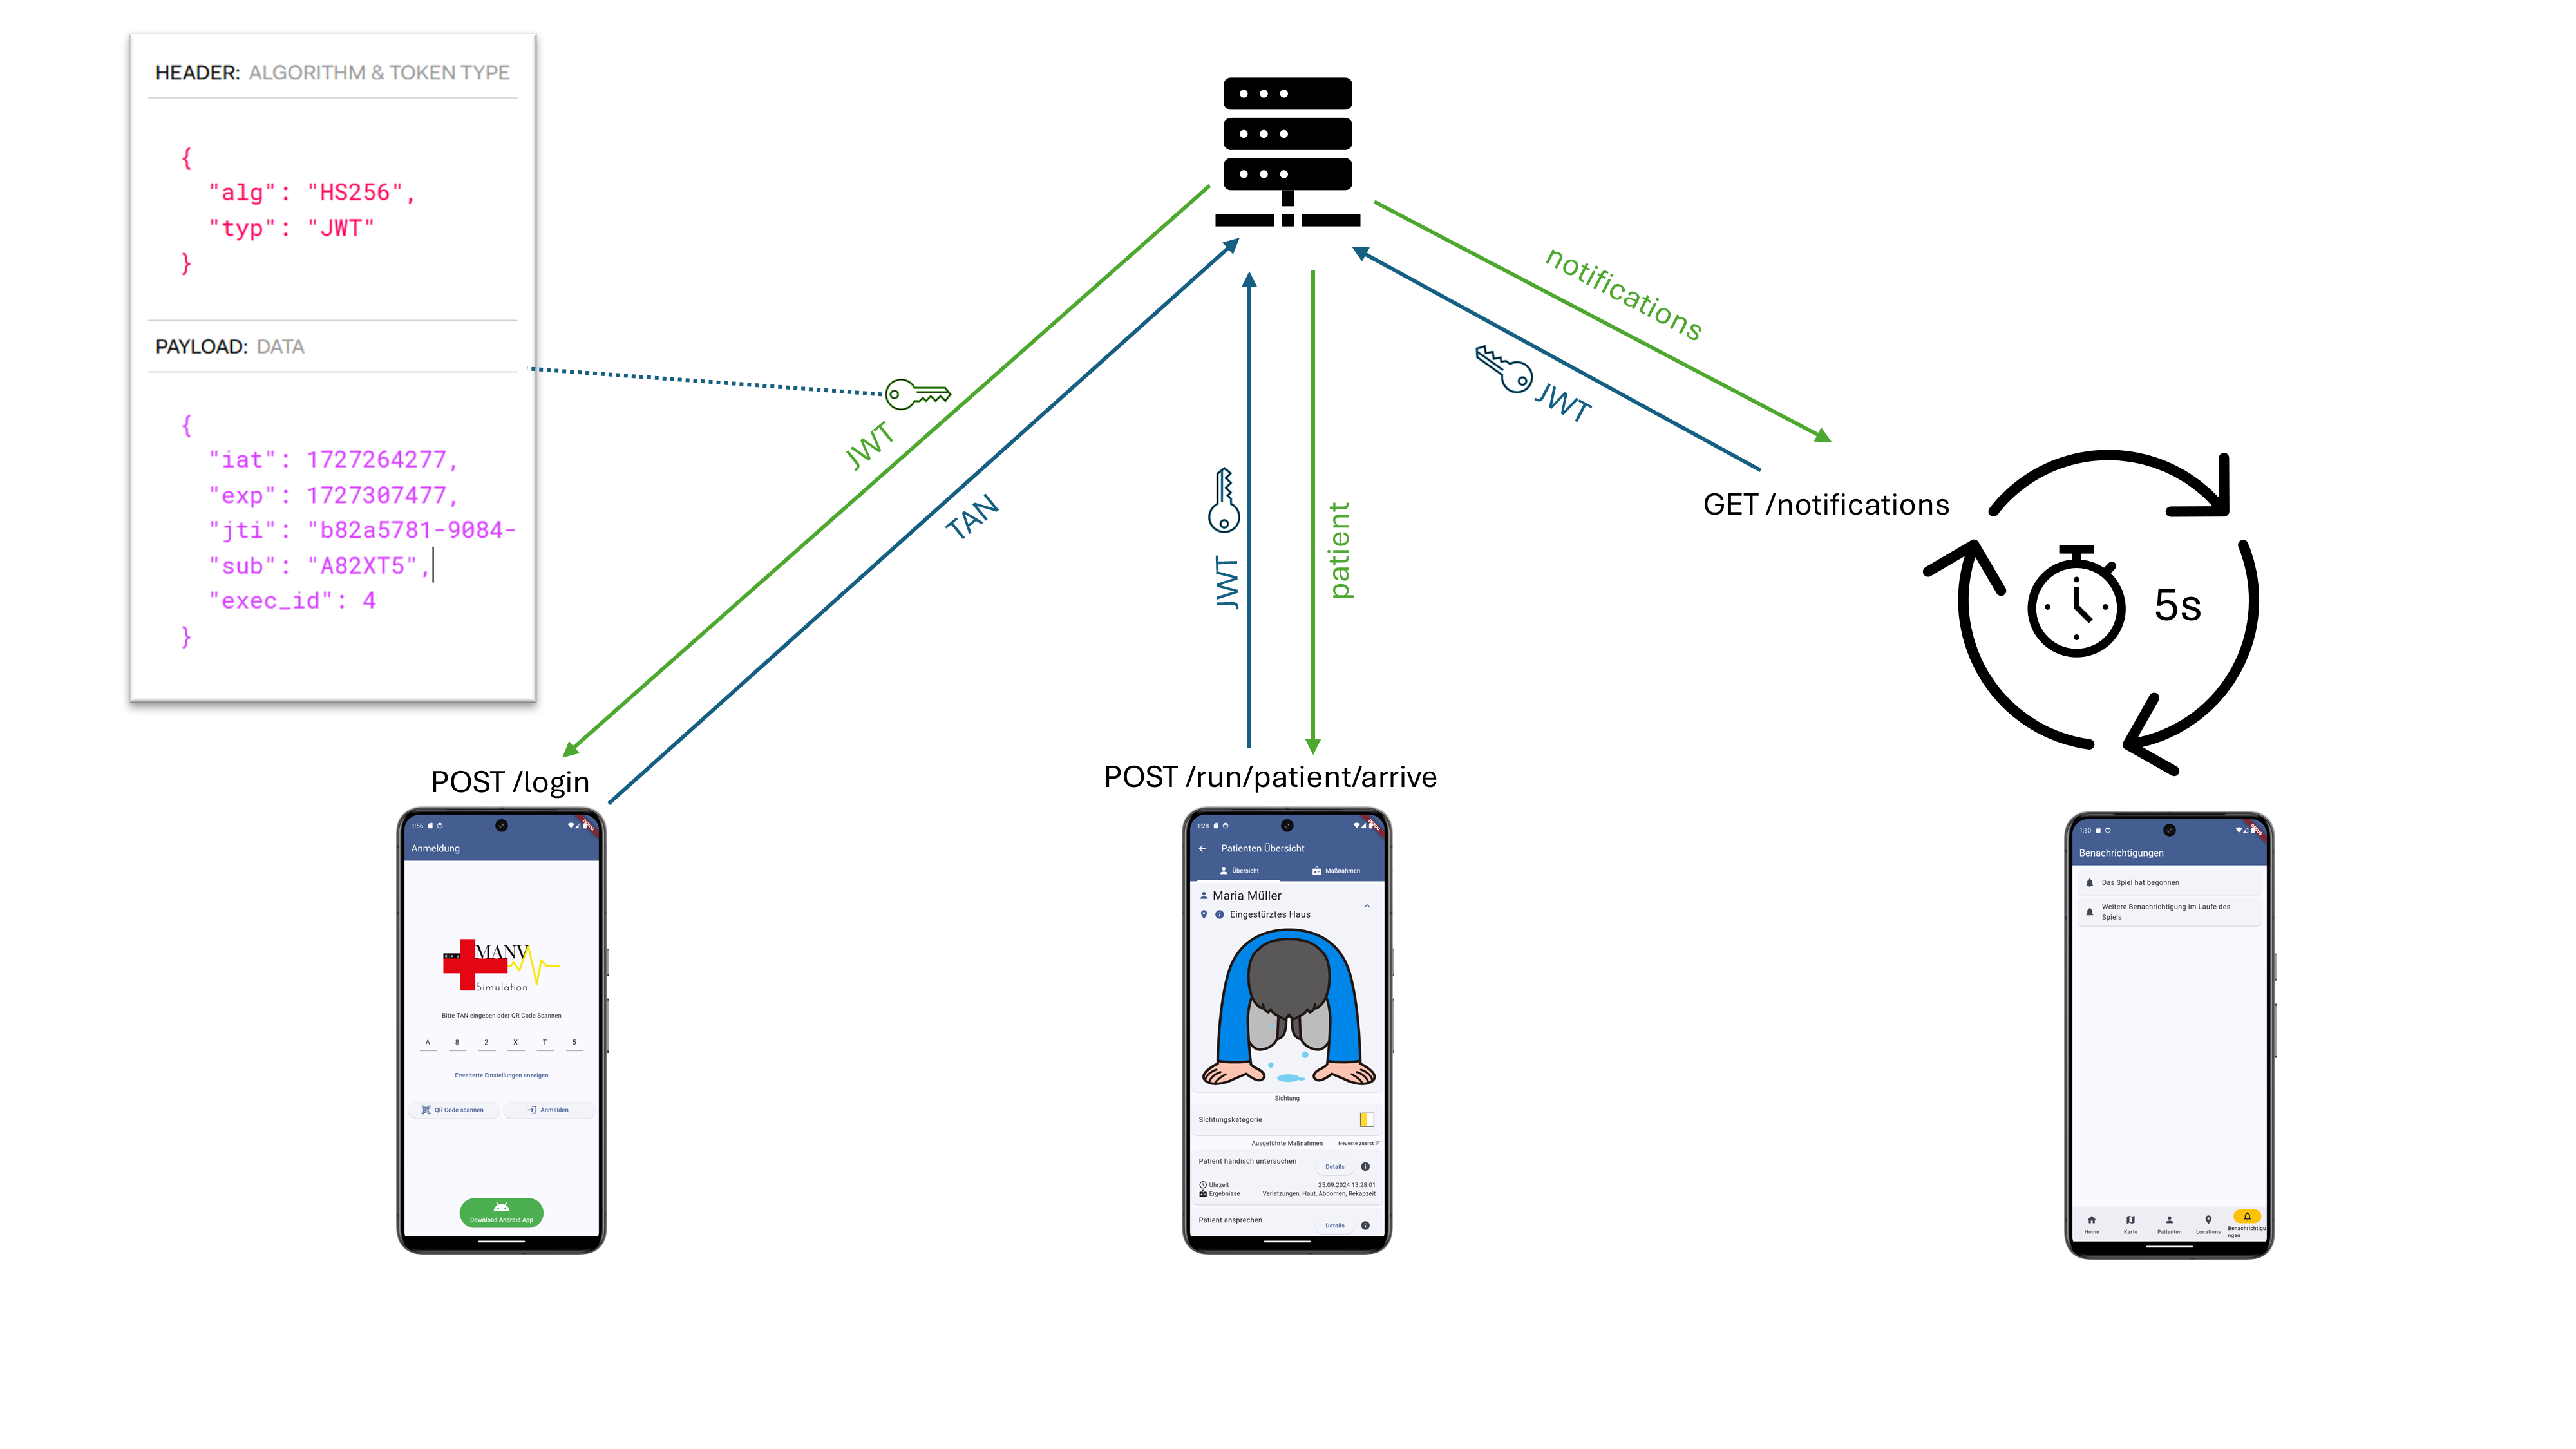
\includegraphics[width=1.0\textwidth]{images/app/api_flow.png}
\end{frame}

\begin{frame}{App - Kommunikation mit Server}
    \vfill
    \begin{figure}
        \centering
        \begin{minipage}{0.3\textwidth}
            \centering
            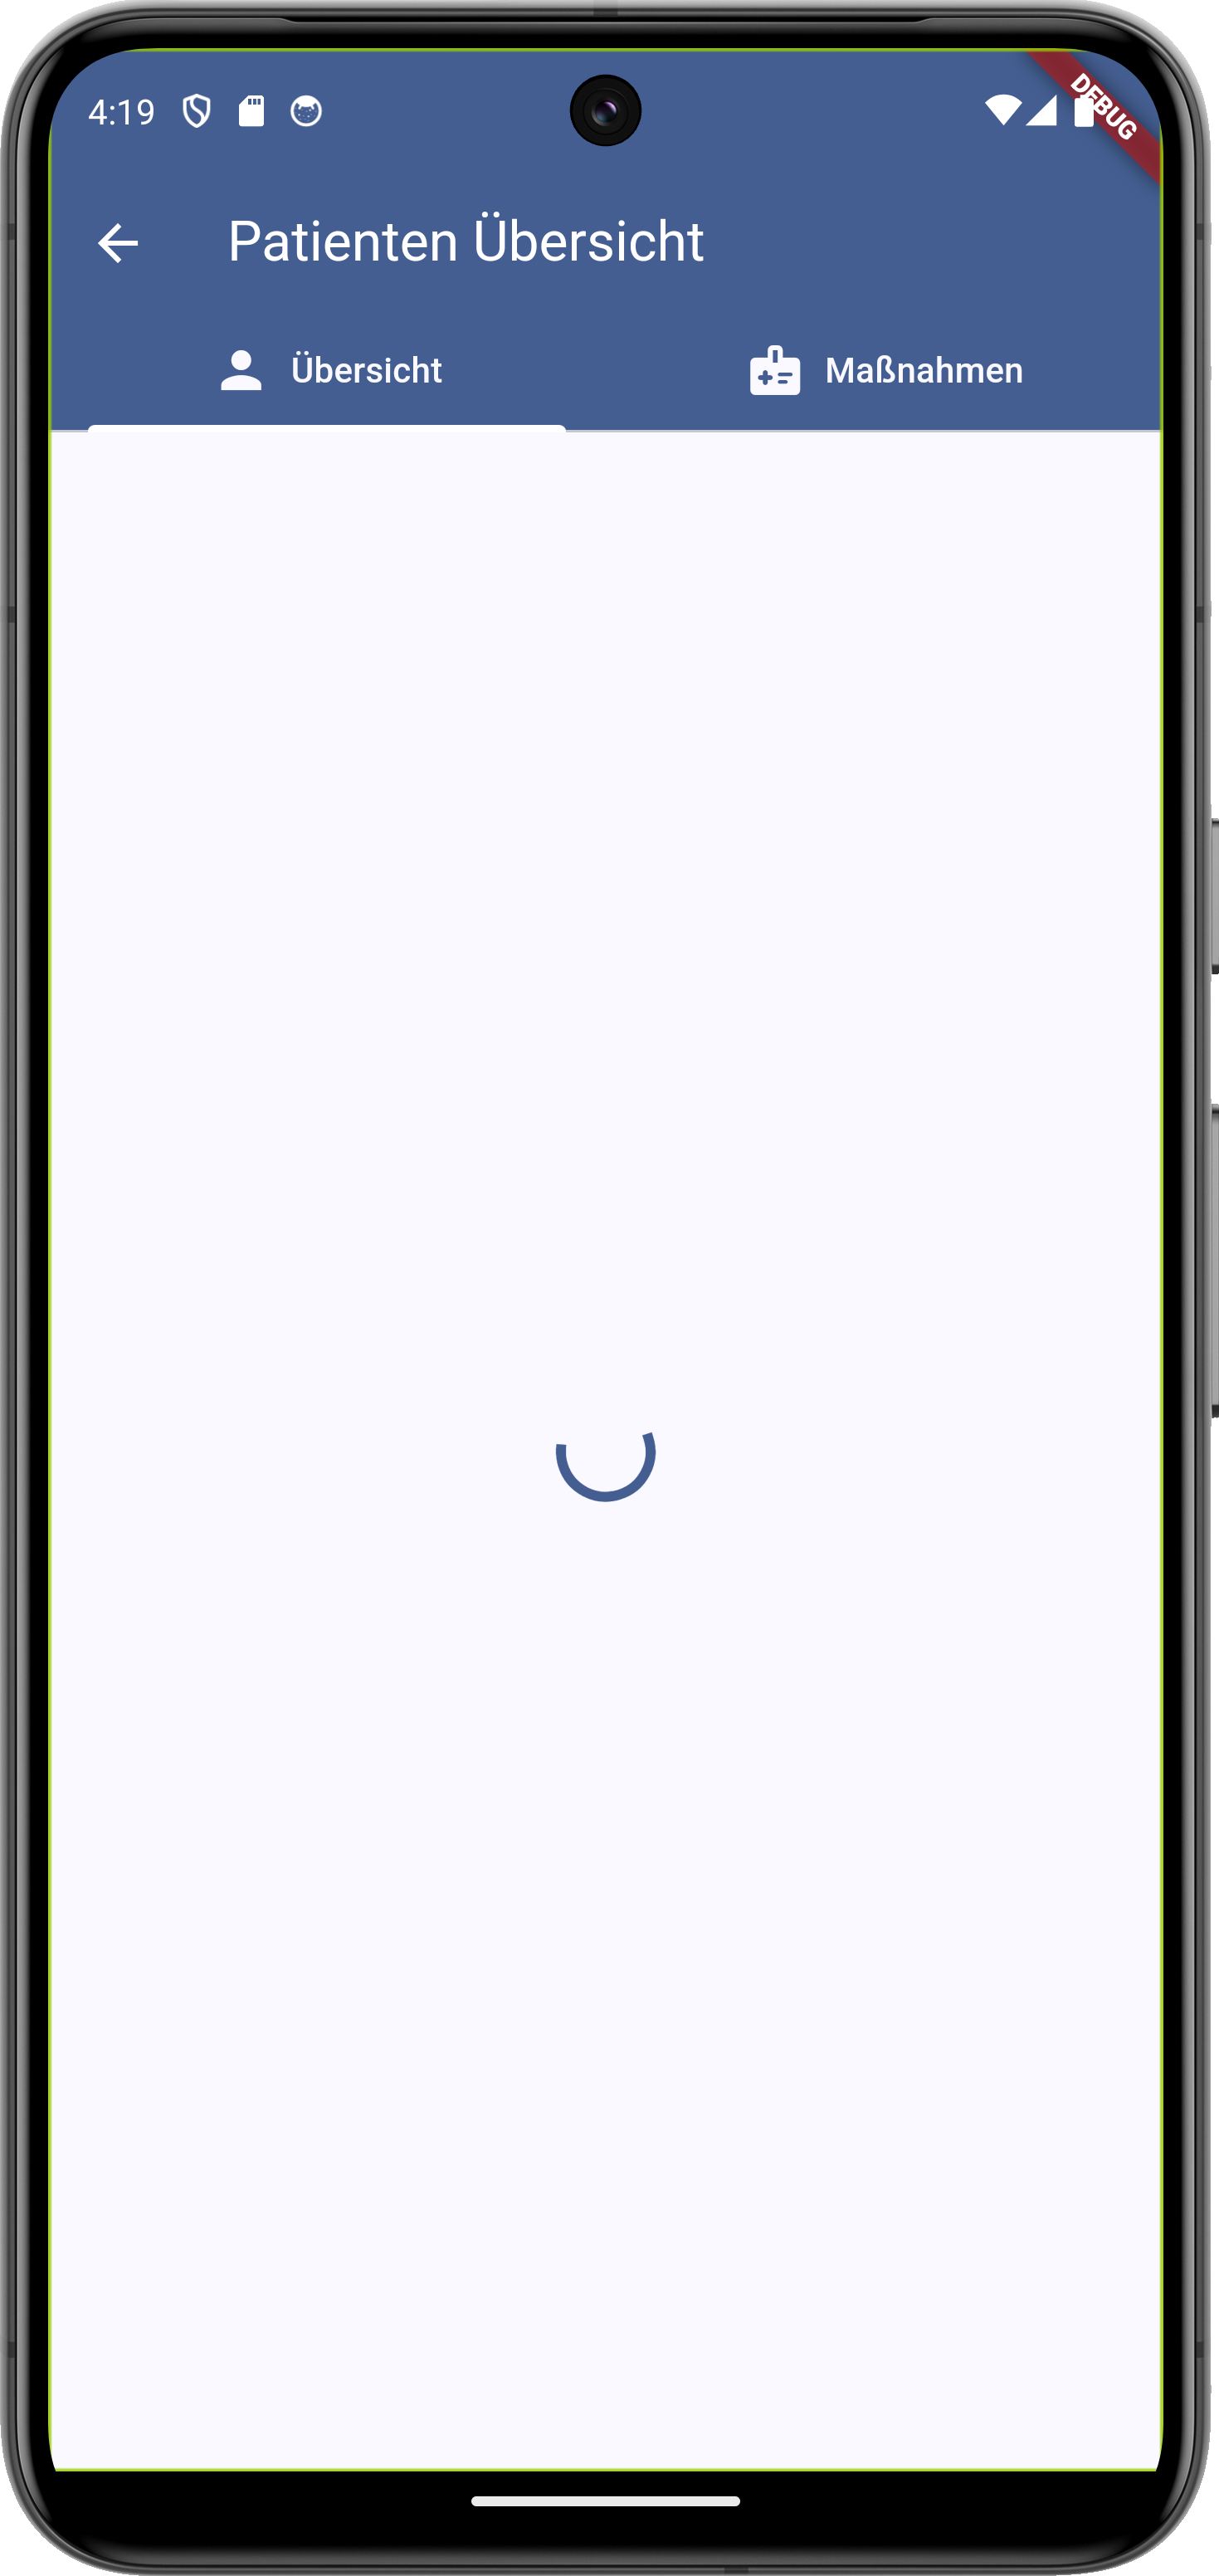
\includegraphics[height=0.8\textheight]{images/app/screenshots/concurrency_loading.png}
            \par{Laden}
        \end{minipage}
        \hspace{0.5cm}
        \begin{minipage}{0.3\textwidth}
            \centering
            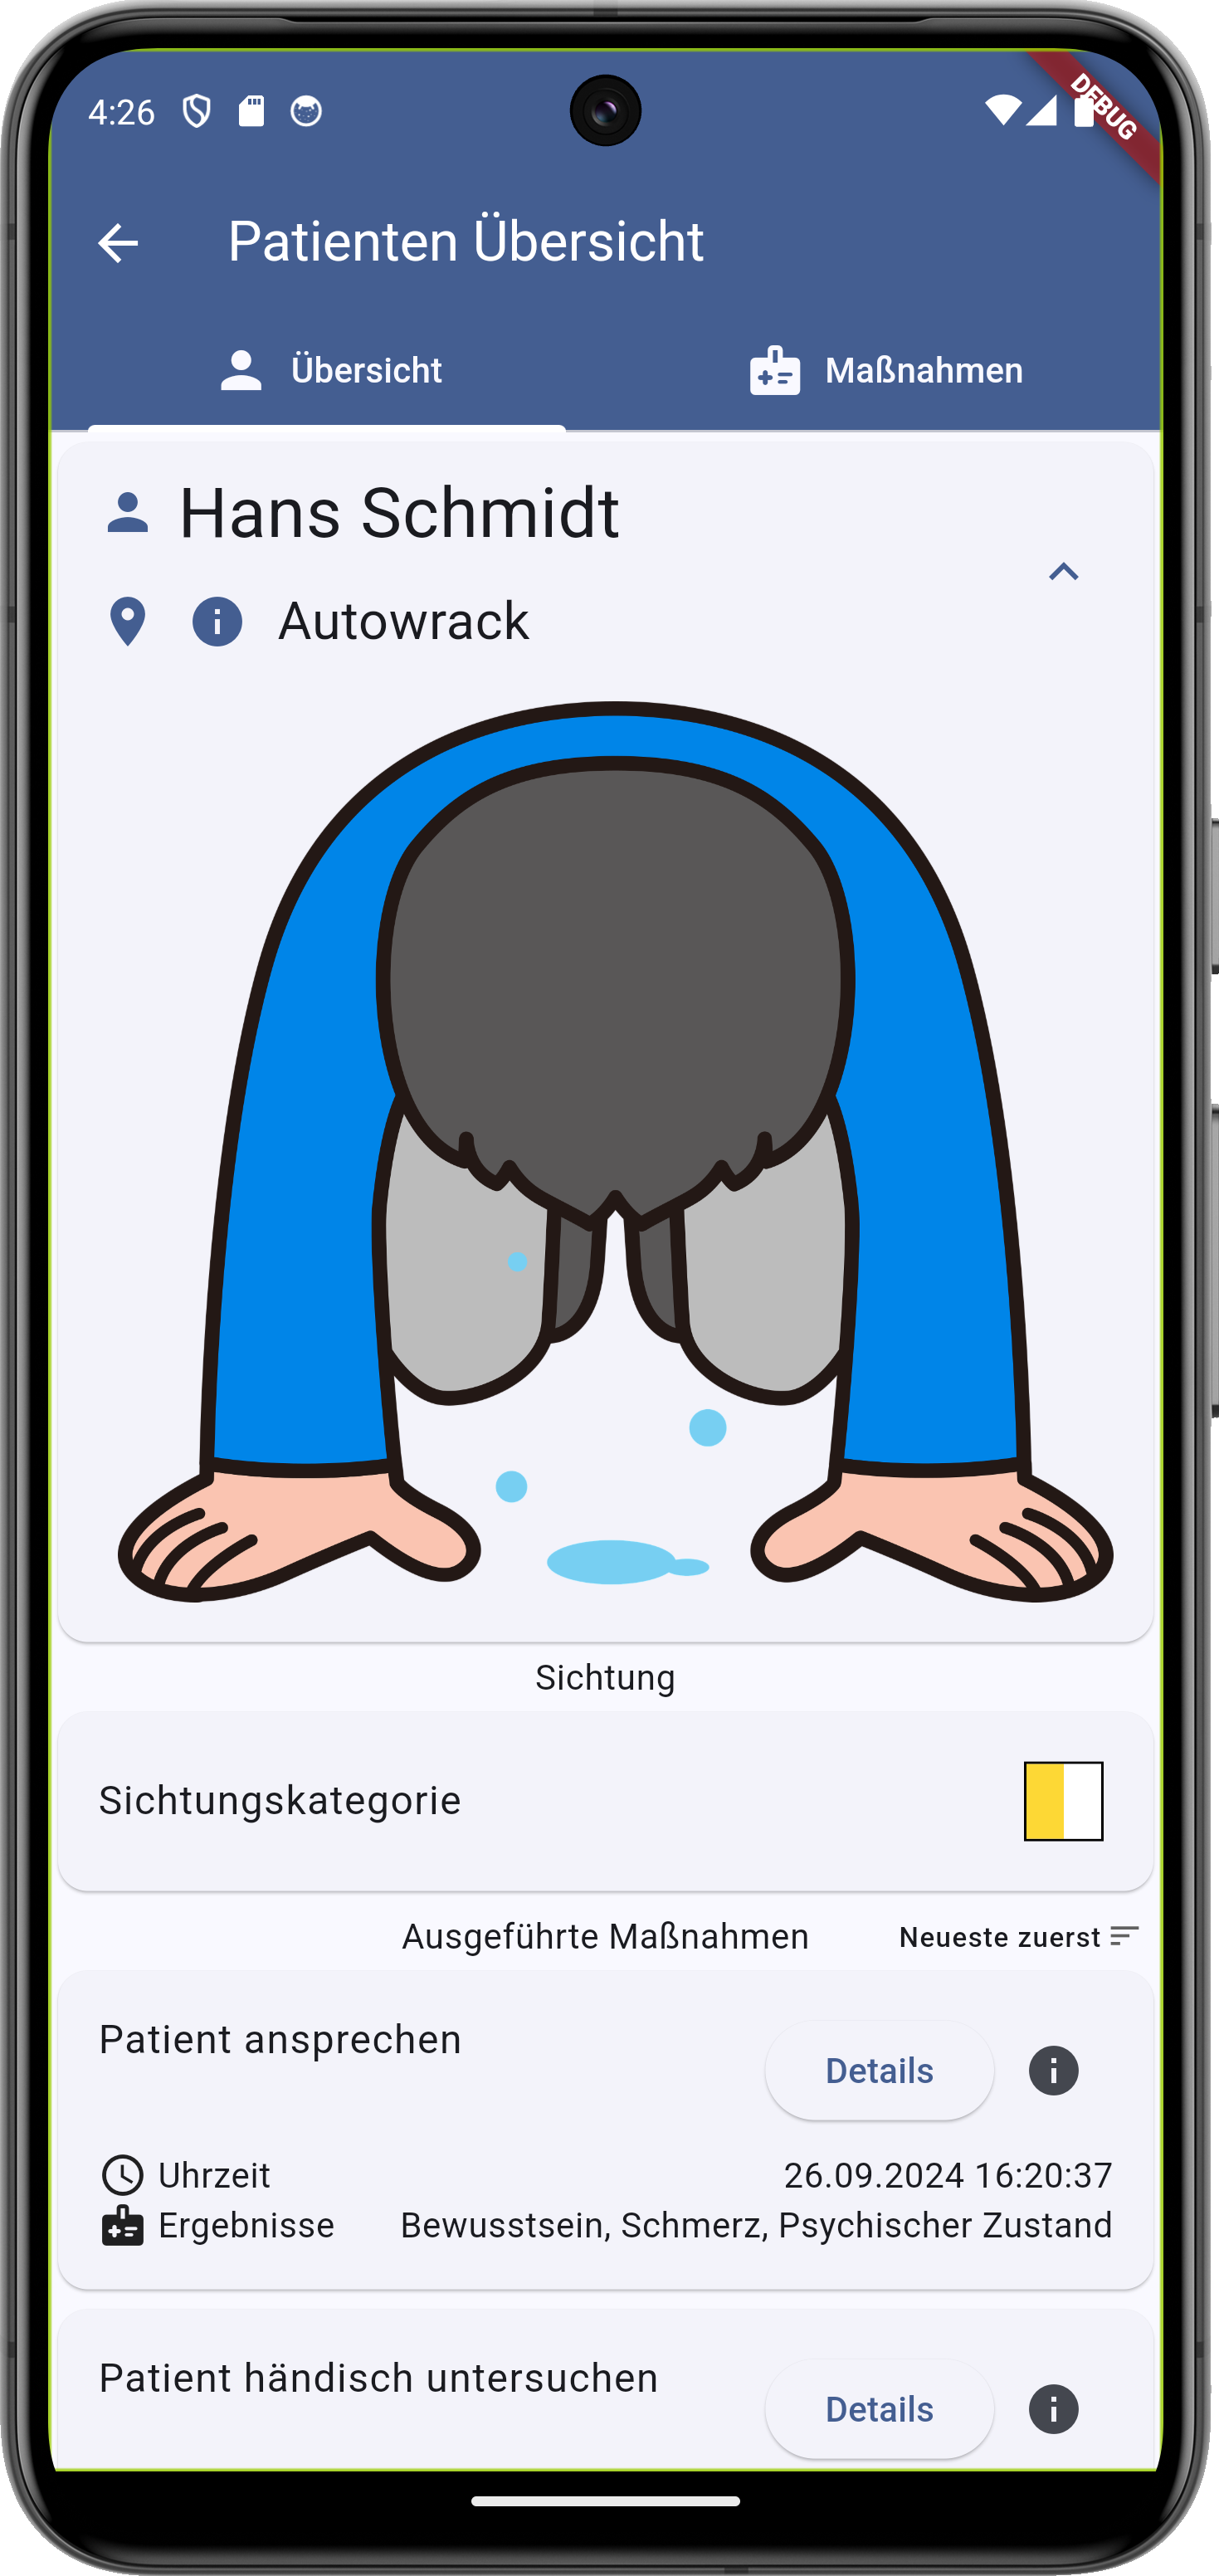
\includegraphics[height=0.8\textheight]{images/app/screenshots/concurrency_ok.png}
            \par{Ereignis}
        \end{minipage}
        \hspace{0.5cm}
        \begin{minipage}{0.3\textwidth}
            \centering
            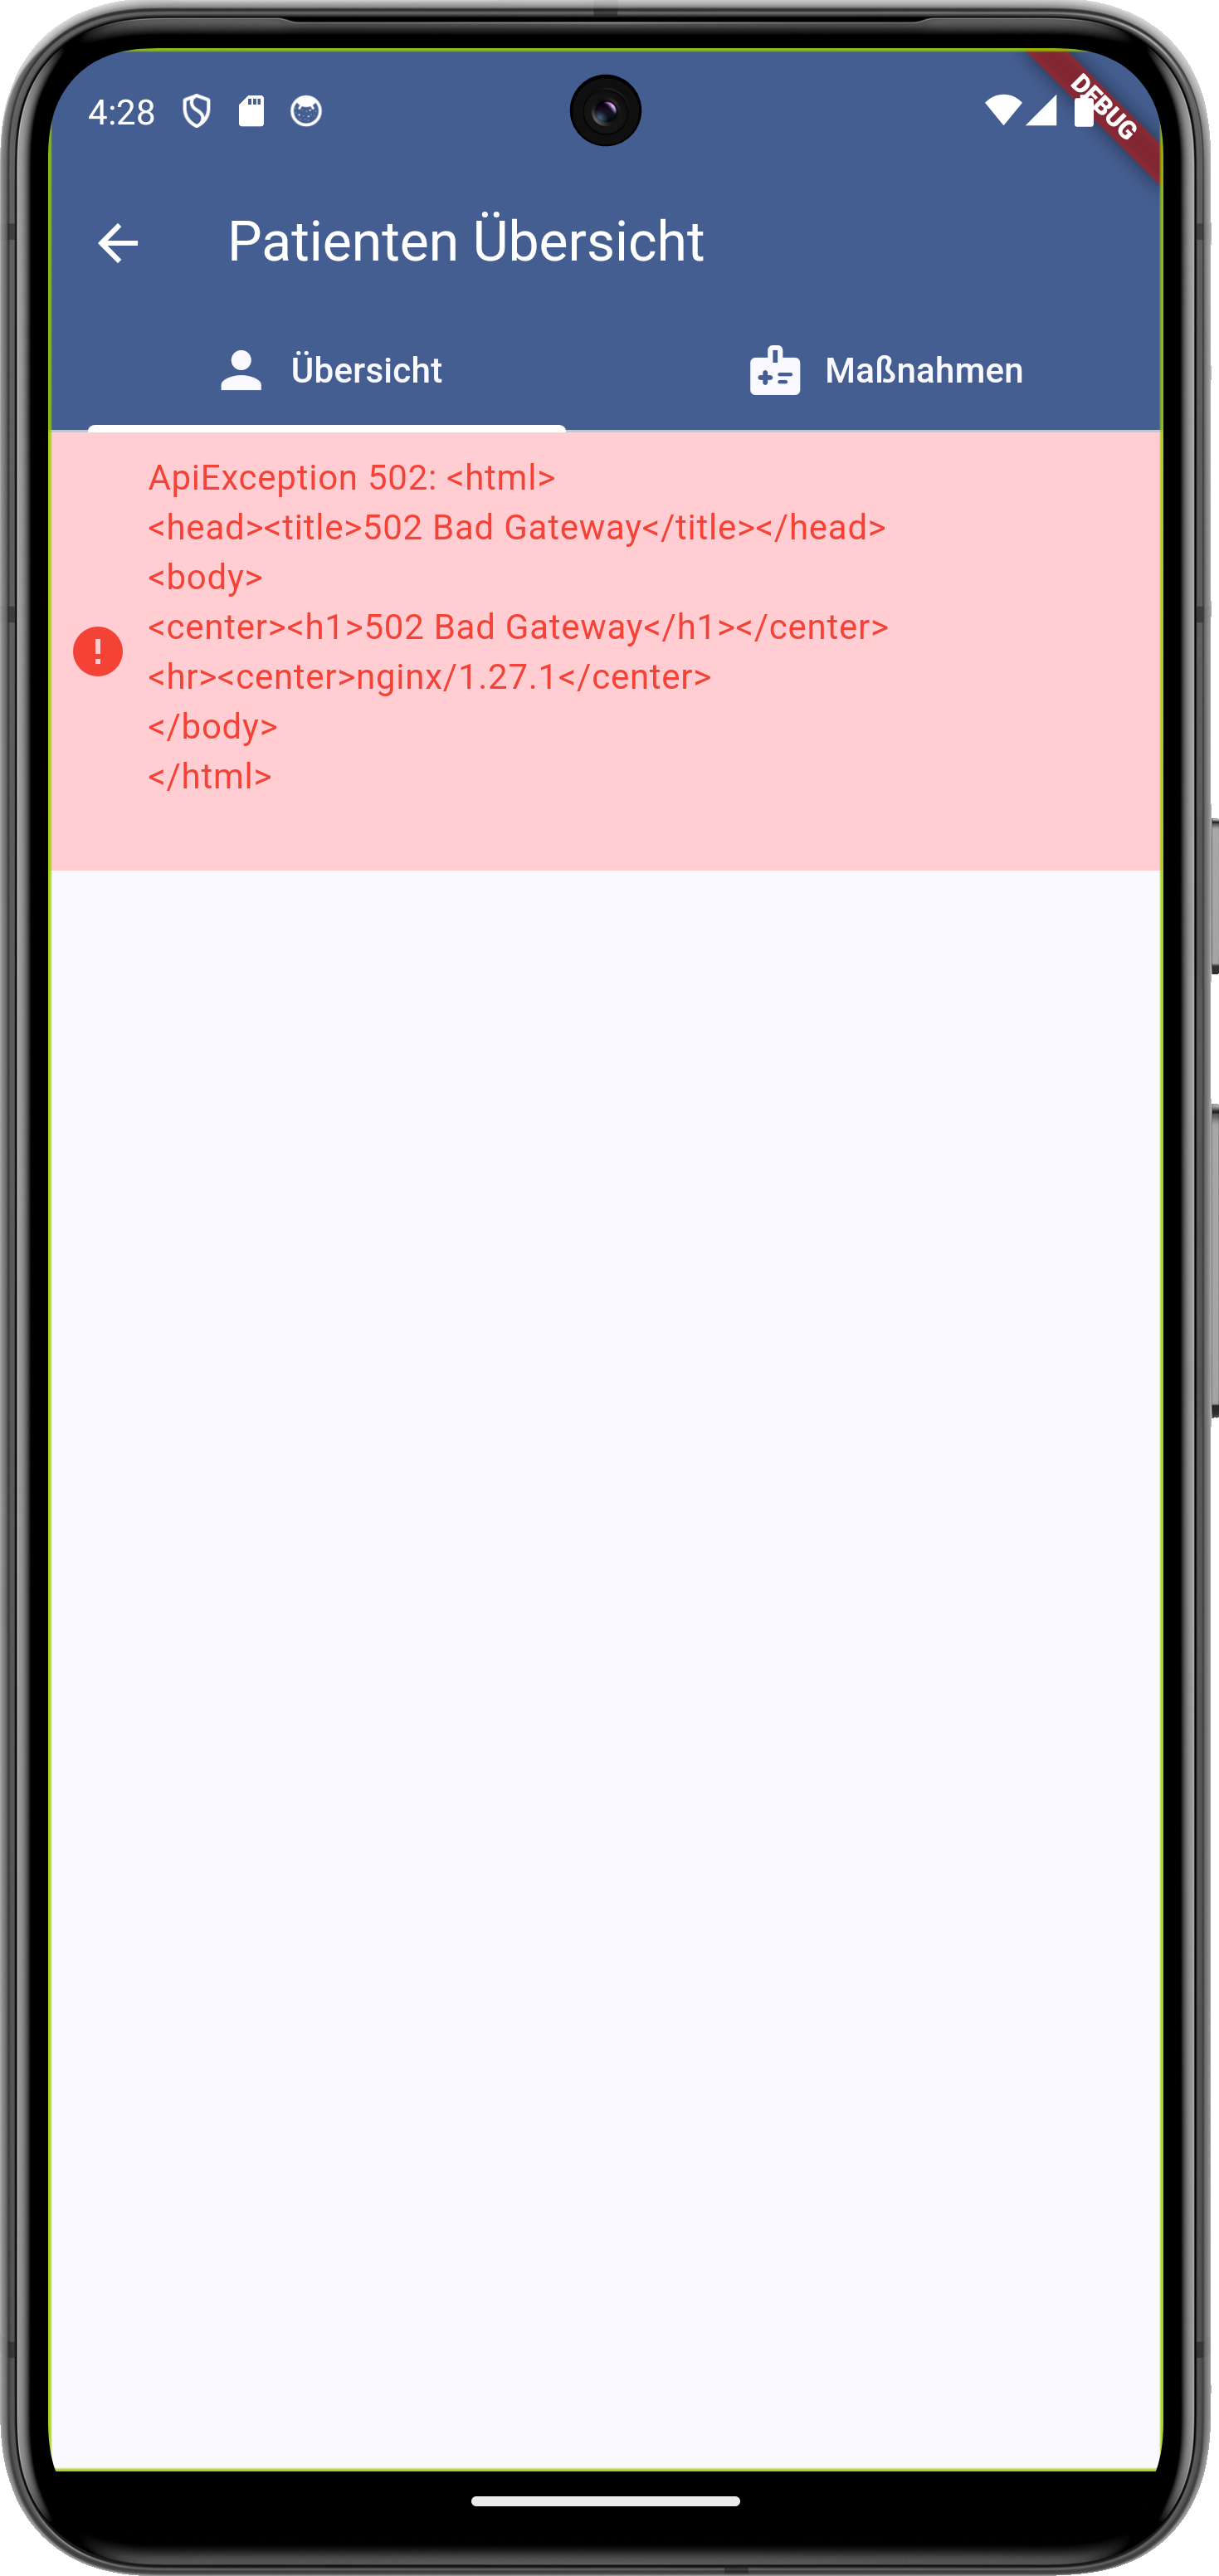
\includegraphics[height=0.8\textheight]{images/app/screenshots/concurrency_error.png}
            \par{Fehler}
        \end{minipage}
    \end{figure}
    \vfill
\end{frame}
